\begin{figure}[tb]
\centering
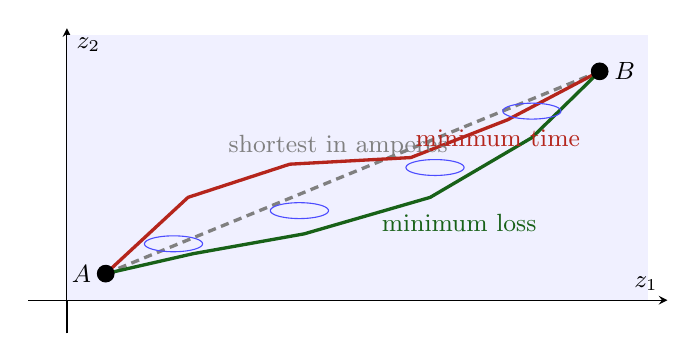
\begin{tikzpicture}[font=\small]
 \begin{axis}[width=.8\linewidth,height=.45\linewidth,axis lines=middle,
  xmin=-.4,xmax=6.2,ymin=-.5,ymax=4.1,ticks=none,xlabel={$z_1$},ylabel={$z_2$},clip=false]
  \fill[blue!6] (axis cs:0,0) rectangle (axis cs:6,4);
  \addplot[gray,densely dashed,very thick] coordinates {(.4,.4)(5.5,3.45)};
  \addplot[BrickRed,very thick] coordinates {(.4,.4)(1.25,1.55)(2.3,2.05)(3.55,2.15)(4.55,2.72)(5.5,3.45)};
  \addplot[ForestGreen!70!black,very thick] coordinates {(.4,.4)(1.3,.7)(2.45,1.0)(3.75,1.55)(4.8,2.45)(5.5,3.45)};
  \addplot[only marks,mark=*,mark size=3pt,black] coordinates {(.4,.4)(5.5,3.45)};
  \node[anchor=east] at (axis cs:.35,.4) {$A$};
  \node[anchor=west] at (axis cs:5.55,3.45) {$B$};
  \node[gray,anchor=south] at (axis cs:2.8,2.0) {shortest in amperes};
  \node[BrickRed,anchor=south west] at (axis cs:3.5,2.17) {minimum time};
  \node[ForestGreen!70!black,anchor=north west] at (axis cs:3.15,1.45) {minimum loss};
  \addplot[blue!70,thin,domain=0:360,samples=50] ({1.1+.30*cos(x)},{.85+.12*sin(x)});
  \addplot[blue!70,thin,domain=0:360,samples=50] ({2.4+.30*cos(x)},{1.35+.12*sin(x)});
  \addplot[blue!70,thin,domain=0:360,samples=50] ({3.8+.30*cos(x)},{2.00+.12*sin(x)});
  \addplot[blue!70,thin,domain=0:360,samples=50] ({4.8+.30*cos(x)},{2.85+.12*sin(x)});
 \end{axis}
\end{tikzpicture}
\caption{Core dynamic message.  Euclidean current length, minimum travel time,
and minimum transient loss select different curves.  The small local speed
bodies show the physical ruler used by the time-optimal path.}
\label{fig:geodesic-core}
\end{figure}
